\chapter{METHODS}
\label{ch:methods}

\section{Motion Correction}

In the previous chapter, we discuss several techniques used to retrospectively correct motion. Motion correction pipelines may use denoising and filtering, but all pipelines begin with volume registration. In this section, we discuss a different approach to volume registration, how it compares to traditional volume registration, and how volume registration fits into a motion correction pipeline. 

%In this section, we discuss the two registration frameworks we apply to our rs-fMRIs: the traditional global volume registration framework and the DAG-based global volume registration framework. The registration frameworks will later be evaluated in comparison to each other, but will also be evaluated in the context of a complete motion correction pipeline. The motion correction pipeline of choice, ICA, will also be discussed in this section.

\subsection{Directed Acyclic Graph Based Volume Registration}

As discussed previously, the major drawback to Friston et al.'s approach to volume registration is that it only minimized the positional differences between the reference volume and the rest of the sequence. This drawback demonstrates an inability for the traditional approach to account for relationships in the patient's position throughout the scan. Intuitively, we know that the patient's position at any volume in the scan is more similar to his position in the immediately previous or subsequent volume than to another randomly chosen volume in the image.

In our proposed framework, we wish to account for these spatiotemporal relationships between temporally neighboring volumes in the sequence. To accomplish this goal, we start by viewing the rs-fMRI sequence as a directed acyclic graph (DAG). A DAG consists of a set of nodes and edges. Each edge has a direction associated with it and connects a pair of nodes. Since a DAG contains no cycles, there is no possible path back to a node once it has been traversed. 

\begin{figure}
\centering
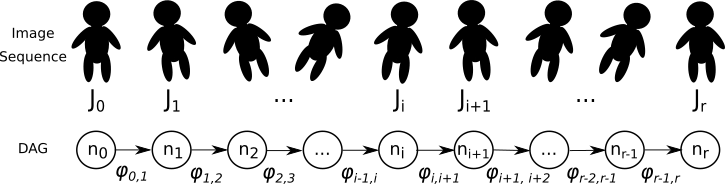
\includegraphics[width=.7\textwidth]{4/dag-chain.png}
\caption{A rs-fMRI can be viewed as a directed acyclic graph where each volume is a node and the edges connect from each volume $i$ to the following volume $i+1$.}
\label{ch4:fig:dag-chain}
\end{figure}

In the case of an rs-fMRI, each volume can be considered a node. The relationship between each pair of temporally neighboring volumes is represented as a directed edge connecting the node for the first volume to the node for the next volume. The acyclic nature of the DAG means that once a patient was in a specific position, he will never return to that exact same position with the exact same neurons firing. The position of the subject and his brain activity as measured by the BOLD signal may be similar in subsequent image volumes, but it will never be precisely the same. The perspectives of an rs-fMRI sequence as a set of images and of the sequence as a DAG can be seen in Figure \ref{ch4:fig:dag-chain}.

The cost of transitioning from one node to the next in our DAG has a parallel representation to the combination of the positional transformation needed to align volume $i$ to volume $i+1$ and the signal change between the volumes. This representation can be written as 

\begin{equation}
J_{i+1} = \phi_{i,i+1} J_i + \delta s_{i,i+1} + \epsilon
\end{equation}

\noindent{where $J_i$ and $J_{i+1}$ are volumes $i$ and $i+1$, $\phi_{i,i+1}$ is a matrix of transformation parameters that must be applied to $J_i$ to achieve the patient’s position in $J_{i+1}$, $\delta s_{i,i+1}$ is the natural change in BOLD signal, and $\epsilon$ is the change in BOLD signal due to motion. Currently, there is no way to estimate the natural change in BOLD signal and the change in BOLD signal due to motion without incorporating additional information about the MRI scanner and the patient that is not included in a rs-fMRI. We simplify our representation of the relationship between two volumes to}

\begin{equation}
J_{i+1} = \phi_{i,i+1} J_i + \epsilon^*
\end{equation}

\noindent{where $\epsilon^*$ is the change in the BOLD signal that cannot be accounted for after aligning the patient’s position in the two volumes. Here, we use the notation $\epsilon^*$ to represent the generic error change in BOLD signal across any pair of volumes.}

After aligning two volumes $i$ and $i+1$, we will then align volumes $i+1$ and $i+2$:

\begin{equation}
\begin{split}
J_{i+2} &= \phi_{i+1,i+2} J_{i+1} + \epsilon^* \\
&= \phi_{i+1,i+2} (\phi_{i,i+1} J_i + \epsilon^*) +\epsilon^*\\
&= \phi_{i+1,i+2} \phi_{i,i+1} J_i + \epsilon^{*'}\\
\end{split}
\end{equation}

Traditional volume registration assumes that 

\begin{equation}
\phi_{i,i+2} = \phi_{i+1,i+2} \phi_{i,i+1}
\end{equation}

\begin{figure}
\centering
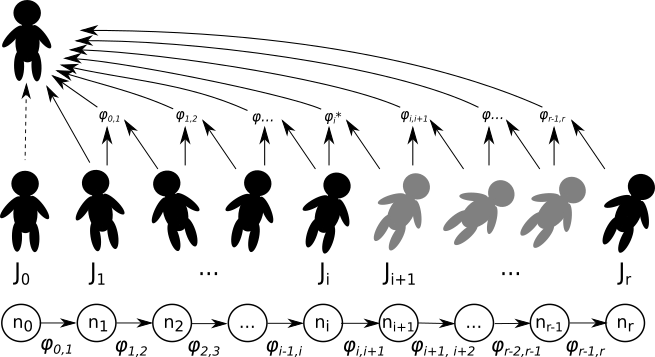
\includegraphics[width=.7\textwidth]{4/dag-registration.png}
\caption{The traditional approach to volume registration in an rs-fMRI sequence consists of registering all volumes in the sequence to a single reference volume.}
\label{ch4:fig:dag-reg}
\end{figure}

\noindent{and calculates $\phi_{i,i+2}$ directly. We argue that this assumption is not true in all cases. Rather than directly calculate $\phi_{0,i}$ and use it to align volume $i$ to the reference volume as the traditional method does, we calculate each component $\phi$ that is a factor of $\phi_{0,i}$. Each component $\phi_{i,i+1}$ is combined with the preceding $\phi_{0,i}$s to recursively align volume $i+1$ to the reference volume without making the large and often inaccurate transformations required by directly calculating $\phi_{0,i+1}$.} This process is outlined in Figure \ref{ch4:fig:dag-reg}.

\subsection{Motion Correction Pipeline}

After performing volume registration to ensure the patient is in the same physical space throughout the image sequence, the image sequence may still contain artifacts due to motion. Many pipelines exist for correcting motion in registered rs-fMRIs. 

\section{Motion Metrics}

In the previous chapter, the gold standard thresholds for rs-fMRI usability were discussed. These thresholds use the FD and DVARs metrics between neighboring volumes. While the FD and DVARs metrics quantify the volume-to-volume motion well, they do not quantify the overall motion contained in the image sequence. Other metrics, such as the Dice coefficient and the correlation ratio, may be useful in quantifying whole-sequence motion.

\subsection{Dice Coefficient}

The Dice coefficient was proposed by Lee R. Dice in 1945 \cite{Dice1945}. Dice examined several existing metrics for measuring association, and finding them lacking, proposed his own ``coincidence index''. His coincidence index measures the association between a number of samples $a$ where condition $A$ is true and a number of samples $b$ where condition $B$ is true:

\begin{equation}
Index = \frac{2h}{a+b}
\end{equation}

In this equation, $h$ represents the number of samples where both conditions $A$ and $B$ are true. His index can take on any value between 1.0 and 0.0 such that a value of 1.0 means that conditions $A$ and $B$ are true for all samples. Similarly, a value of 0.0 means that conditions $A$ and $B$ are never both true for any sample. While this index is a count of samples that meant both conditions and not a true probability, Dice suggests that the chi-squared test can be used to determine if the combinations of conditions in the samples from a set of data is meaningful or due to random chance. 

Many medical imaging researchers have adapted the Dice coefficient to measure the overlap between pairs of images. %The images could be manual and automatic segmentations of the same area, segmented images registered to each other, or ELEPHANTS.
Zijdenbos et al. trained an artificial neural network to semiautomatically segment brain MRIs and compared the generated segmentations to manual segmentations using the Dice coefficient \cite{Zijdenbos1994}.
Zou et al. used the Dice similarity coefficient in their analysis of the reproducibility of manually segmented MRIs and the accuracy of automatic segmentations of the same images for prostate and brain tumor datasets \cite{Zou2004}. 
Liao et al. used it to measure the accuracy of a volume registration framework for aligning manual segmentations of multiple organs in fetal images \cite{Liao2016}. Bharatha et al. performed a study on pre- and intra-operative images of the prostate. They segmented the images, generated deformable finite element models of the segmentations, and used the Dice coefficient to compare the registered segmentations and finite element models \cite{Bharatha2001}.

%The global volume registration techniques were applied to all 17 resting-state BOLD MR images. After the registrations, each subject had three sequences associated with it: the original sequence, the sequence registered using the traditional framework, and the sequence registered using the DAG-based framework. The globally registered images were compared to each other in terms of correlation ratios between all volumes in the sequence as well as FD and DVARS between temporally neighboring volumes. 

It should be noted that the Dice coefficient as used in these contexts is a measure of similarity of items from two categories which take on binary conditions. Additionally, all studies mentioned in the previous paragraph require a manually segmented gold standard image to which the automatic segmentations or registered images can be compared. Medical images do not naturally have binary values, nor is it always reasonable to obtain manual segmentations of all images in a dataset. In cases where a good image segmentation cannot be obtained, other similarity metrics such as mutual information and cross correlation should be used instead.

\subsection{Correlation Ratio Matrix}

The correlation ratio is an asymmetrical, spatially informed measure of the overlap between images. It is different from other similarity metrices in that a lower correlation ratio indicates a better alignment between two images rather than a worse alginment. 

The earliest symbolic representation of the correlation ratio is 

\begin{equation}
\label{ch4:eq:cr-orig}
\eta = \frac{\Sigma}{\sigma_y} = \frac{\sqrt{\frac{\sum(n_x(\overline{y}_x - \overline{y})^2)}{N}}}{\sigma_y}
\end{equation}

where $n_x$ is the number of samples in any one set $x$, $\overline{y}_x$ is the average of the samples in $x$, $\overline{y}$ is the average of all samples in all sets, $\sigma_y$ is the standard deviation of all samples in all sets, and $N$ is the total number of samples across all sets \cite{Rugg1917}. The meaning of this equation was simplified by Ayres, who describes it as ``the ratio between two standard deviations'' \cite{Ayres1920}. In Equation \ref{ch4:eq:cr-orig}, the numerator is the standard deviation of a single set of samples with respect to all sets of samples, and the denominator is the standard deviation of all sets of samples. The process of calculating the individual components of this equation are outlined in \cite{Rugg1917}.

The correlation ratio was proposed for use in medical imaging applications in 1998 and compared to other similarity metrics. Roche et al. provide an example of algining two black images, one with a uniform gray stripe and the other with a horizontal gray gradient, such that the overlap between the two images is maximally similar \cite{Roche1998a}, \cite{Roche1998}. They show that the mutual information metric has a maximum value at every translation of an integer number of pixels while the correlation ratio had a maximum value at one single alignment. They apply the correlation ratio to MR images as well as computed tomography and positron emission tomography images. Their experiments suggest that in the context of multimodal registration, the correlation ratio balances accuracy and robustness.

In the context of medical imaging, the correlation ratio measures the functional dependence between a pair of images $X$ and $Y$. The correlation ratio of $Y$ given $X$ is

\begin{equation}
\eta(Y|X) = \frac{Var[E(Y|X)]}{Var(Y)}
\end{equation}

This equation is comparing the energy of $Y$ in $X$ to the total energy of $Y$. If $X$ and $Y$ overlap in area $\Omega$, the number of pixels in that area is $N = Card(\Omega)$. Since $X$ is known, it can be divided into sets of pixels $\Omega_i$ where each set is comprised of locations in $\Omega$ where the pixels $X$ have the same value $i$. 

Because the correlation ratio shows is a strong metric for measuring the similarity between two images, we suggest using it to quantify the similarity between all volumes in an image sequence. We choose to refer to this metric as the correlation ratio matrix. For a sequence of length $l$, the correlation ratio matrix $M$ is a square, asymmetrical matrix of size $l*l$. Each cell in $M$ is calculated as

\begin{equation}
M_{i,j} = \eta(J_i, J_j) = \frac{Var[E(J_i|J_j)]}{Var(J_i)} =  \frac{\sqrt{\frac{\sum |J_i|(\overline{J_i} - \overline{J_i \cap J_j})^2)}{|J_i \cap J_j|}}}{\sigma_{J_i \cap J_j}}
\end{equation}

where $J_i$ and $J_j$ are volumes $i \in l$ and $j \in l$ in the sequence, respectively, $|*|$ indicates the number of voxels in the operand, $\overline{*}$ indicates the average of the voxel values in the operand, and $J_i \cap J_j$ is the volume of space where images $J_i$ and $J_j$ intersect. %In volume registration, the computer assumes the entire contents of $J_i$ and $J_j$ intersect provided they are the same size (in voxels), which somewhat simplifies 

Since the matrix $M$ is quite large, using statistics describing $M$ rather than $M$ itself can simplify analyses. On the other hand, the whole matrix $M$ may be more comprehensively analyzed using statistical tests such as the $t$-test.

\section{Analysis of Motion Correction}

The purpose of motion correction is to remove noise from valuable signal in an image. The amount of motion removed from an image can be quantified using the FD and DVARS usability thresholds, but that analysis does not explain how volume registration and motion correction techniques generalize to larger populations. 

Statistical analyses can be used to identify general trends within a data set. Statistical tests can be used to compare images before and after motion correction within each subject population. They can also indicate the degree of significance of the effects of volume registration and motion correction. 

\section{Motion Patterns} 

We suggest that the ways that patients move are specific to certain patient groups. For example, fetal patients live suspended in amneotic fluid and as such are subject to different physical constraints than patients in other age groups. Neonatal patients are often scanned using a ``feed and bundle'' protocol, which often results in them sleeping through the scan. However, neonatal patients sometimes wake up during the scan. The way a baby woken up from a nap moves is different from how a fidgety preadolescent moves, though the terminology to define how these movement patterns differ is somewhat lacking. 

There is also a chance that patients within the same age group move differently possibly due to their cognitive state. Preadolescents who have ADHD likely become bored and fidgety in the MR scanner at different rates then their non-ADHD counterparts. Adults suffering from dementia may have more difficulty remaining still for the duration of a scan than adults with similar demographics and no dementia.

These patterns are essentially signals specific to different categories of patients. Machine learning techniques are useful for identifying patterns in signals from different sources. Unsupervised learning techniques group samples from a population based on the patterns in their features. The results of unsupervised clustering algorithms can be visualized and analyzed to determine how the computer chose each group of samples. 

Another approach to analyzing these signals is regression. Regression models the relationships between a set of independent features and an outcome or set of outcomes. For example, the linear regression could be used to evaluate the relationship between motion metrics and the severity of neurodevelopmental outcomes or patient age. 

In addition to machine learning and regression, other techniques from the biomedical imaging and computer vision domains may be used. Supervised machine learning models may also be trained to predict a clinical or behavioral outcome based on a patient's image features.

\section{Implementation: Tools and Libraries}

The registration frameworks described in this section were implemented in Python using the nipype (Neuroimaging in Python Pipelines and Interfaces) library \cite{Gorgolewski2011}. Affine volume registration was performed using ANTs (Advanced Normalization Tools) \cite{Avants2014}. The metric used to estimate the dissimilarity between the pairs of volumes being registered was cross-correlation with a local window size of 5 voxels. 

To calculate metrics, we used several existing tools. FLIRT (FMRIB’s Linear Image Registration Tool) was used to calculate the correlation ratio between each possible pair of volumes in the sequences \cite{Jenkinson2001} \cite{Jenkinson2002}. We then used the average and standard deviation of the correlation ratio distribution of each image to compare the images. We calculated the FD and DVARS metrics defined by Power et al. using the FSLMotionOutliers tool \cite{Power2012}. These metrics were calculated for each image and were used for evaluation of the efficacy of the registration frameworks.